\section{Kvantevandringer}

\subsection{Grover's algoritme og metoden av amplitude amplifikasjon}

    Grover's algoritme løser problemet med ustrukturert søk, og teknikken amplitude amplifikasjon som den bruker er av stor interesse. Problemet går som følger: Tenk at man er gitt en bistring med $N=2^n$ bits, hvor $t$ bits er satt til 1. Finn minst 1 bit som har verdi 1. Dette problemet kan åpenbart løses i "worstcase"\ lineær tid med konstant minne ved å randomisert iterere gjennom alle bitene og sjekke om de er 1 eller 0. Om den er 1 kan man terminere programmet, og returnere den posisjon som ga 1. Grover's algoritme har en kvadratisk hastighetsøkning på dette problemet, og man kan dermed løse det i worst case kvadratisk tid.

    For å beskrive problemet med et fysisk kvantesystem trenger vi å oversette problemet først. La $(b_k)_N$ være bitstringen med lengde N, definer så orakelet $\mathcal{O}_{(b_k)_N}:\mathbb{C}^{2^n} \otimes \mathbb{C}^2 \rightarrow \mathbb{C}^{2^n} \otimes \mathbb{C}^2$ til å merke målbiten hvis registerbiten var en løsning. Dette vil si at hvis $\mathcal{O}_{(b_k)_N}(|r\rangle\otimes |0\rangle) = |r\rangle\otimes |1\rangle$ så følger det at $b_r = 1$. For å fullføre Grover's algoritme trenger man matrisen $R$ som flipper fortegnet til registeret hvis den ikke er tilstanden $|0\rangle^{\otimes n}$.
    \begin{center}
        \begin{math}
            R = \begin{pmatrix}
                1 & 0 & ... \\
                0 & -1 & ... \\
                \vdots & \vdots & \ddots
            \end{pmatrix}
            %= 2|0\rangle\langle 0| - I
        \end{math}
    \end{center}

    En Grover iterate $\mathcal{G}$ er definert som 
    \begin{align*}
        \mathcal{G}=H^{\otimes n}RH^{\otimes n}\mathcal{O}_{(b_k)_N, \pm}.
    \end{align*}
    
    Gorver's algoritme er komposisjonen av operatorene $G = M\mathcal{G}^k\circ H^{\otimes n}$, hvor $M$ er en projektiv måling, og $k$ er en konstant. Man skal da kunne fastslå med en høy sannsynlighet at målingen gir deg posisjonen til en bit i $(b_k)_N$ som er $1$. For å finne denne $k$-en som man bruker for å kjøre algoritmen trenger vi å se på metoden av amplitude amplifikasjon.

    Definer tre tilstander hvor $t$ er antall $1$-ere i $(b_r)_N$ 
    \begin{align*}
        u & = H^{\otimes n}|0\rangle^{\otimes n}\\
        G & = \frac{1}{\sqrt{t}}\Sigma_{|r\rangle \mid b_r = 1}|r\rangle\\ 
        B & = \frac{1}{\sqrt{N-t}}\Sigma_{|r\rangle\mid b_r = 0}|r\rangle
    \end{align*}. 

    \begin{figure}
        \caption{Grover's algoritme}
        \begin{center}
            \begin{subfigure}[b]{0.46\textwidth}
                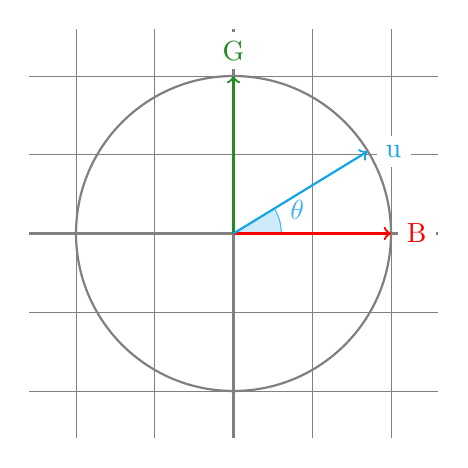
\begin{tikzpicture}[scale=2]
                    \draw[step=.5,gray,very thin] (-1.3,-1.3) grid (1.3,1.3);
                    \draw[gray, thick] (0,0) circle (1);
                    \draw[gray, thick] (1.3, 0) -- (-1.3, 0);
                    \draw[gray, thick] (0, 1.3) -- (0, -1.3);
                    \draw[ForestGreen, thick, ->] (0,0) -- (0, 1) node[above=2pt, fill=white] {G};
                    \draw[Cerulean!80!White, thick] (0.3, 0) arc (0:30:0.3) node[right=2pt] {$\theta$};
                    \fill[Cerulean!20!White] (0,0) -- (0.3, 0) arc (0:30:0.3) -- (0,0);
                    \draw[Red, thick, ->] (0,0) -- (1,0) node[right=2pt, fill=white] {B};
                    \draw[Cerulean, thick, ->] (0,0) -- (0.85,0.52) node[right=3pt, fill=white] {u};
                \end{tikzpicture}
                \caption{Initiell tilstand}
                \label{fig:Grover init}
            \end{subfigure}
            \begin{subfigure}[b]{0.46\textwidth}
                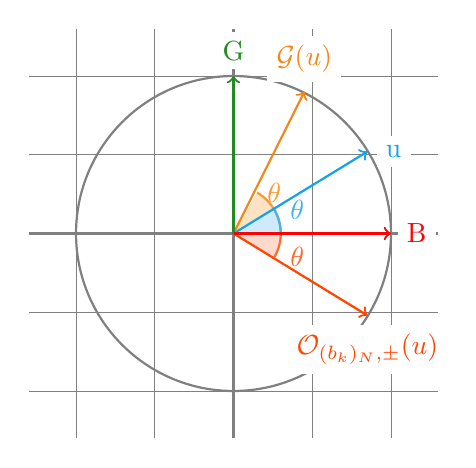
\begin{tikzpicture}[scale=2]
                    \draw[step=.5,gray,very thin] (-1.3,-1.3) grid (1.3,1.3);
                    \draw[gray, thick] (0,0) circle (1);
                    \draw[gray, thick] (1.3, 0) -- (-1.3, 0);
                    \draw[gray, thick] (0, 1.3) -- (0, -1.3);
                    \fill[BurntOrange!20!White] (0,0) -- (0.3, 0) arc (0:60:0.3) -- (0,0);
                    \fill[Cerulean!20!White] (0,0) -- (0.3, 0) arc (0:30:0.3) -- (0,0);
                    \fill[OrangeRed!20!White] (0,0) -- (0.3, 0) arc (0:-30:0.3) -- (0,0);
                    \draw[BurntOrange!80!White, thick] (0.3, 0) arc (0:60:0.3) node[right=0pt] {$\theta$};
                    \draw[Cerulean!80!White, thick] (0.3, 0) arc (0:30:0.3) node[right=2pt] {$\theta$};
                    \draw[OrangeRed!80!White, thick] (0.3, 0) arc (0:-30:0.3) node[right=2pt] {$\theta$};
                    \draw[Cerulean, thick, ->] (0,0) -- (0.85,0.52) node[right=3pt, fill=white] {u};
                    \draw[BurntOrange, thick, ->] (0,0) -- (0.45,0.9) node[above=3.2pt, fill=white] {$\mathcal{G}(u)$};
                    \draw[OrangeRed, thick, ->] (0,0) -- (0.85,-0.52) node[below=3pt, fill=white] {$\mathcal{O}_{(b_k)_N,\pm}(u)$};
                    \draw[ForestGreen, thick, ->] (0,0) -- (0, 1) node[above=2pt, fill=white] {G};
                    \draw[Red, thick, ->] (0,0) -- (1,0) node[right=2pt, fill=white] {B};
                \end{tikzpicture}
                \caption{En Grover iteration}
                \label{fig:Grover en}
            \end{subfigure}
        \end{center}
    \end{figure}
    
    Man kan se at $G$ (Good) og $B$ (Bad) vektorene er ortogonale, ettersom de er en sum av ortogonale vektorerer. I det 2 dimensjonale underrommet av $\mathbb{C}^{2^n}$ utspent av $G$ og $B$, finner man vektoren $u$.
    \begin{align*}
        u & = \frac{1}{\sqrt{N}}\Sigma_{|r\rangle}|r\rangle = \frac{\sqrt{t}}{\sqrt{N}}G + \frac{\sqrt{N-t}}{\sqrt{N}}B \\
        & = \sin\circ\arcsin(\frac{\sqrt{t}}{\sqrt{N}})G+\cos\circ\arcsin(\frac{\sqrt{t}}{\sqrt{N}})B \\
        & = \sin(\theta)G+\cos(\theta)B
    \end{align*}
    Her er $\theta = \arcsin(\frac{\sqrt{t}}{\sqrt{N}})$. Vi ønsker nå å manipulere tilstanden til $u$ i underrommet utspent av $G$ og $B$ for å maksimere $\sin(\theta)$. Dette vil maksimere sannsynligheten for at algoritmen avslutter i en tilstand hvor man har maksimal sjanse for å måle en qubit som er merket. La $\alpha:\mathbb{R}$ være en vinkel og $T = \sin(\alpha)G+\cos(\alpha)B$ være en tilstand. For å se hva orakelet gjør med $T$ kan vi se på hva den gjør med $G$ og $B$. 
    \begin{align*}
        & \mathcal{O}_{(b_k)_N, \pm}(B) = B \\
        & \mathcal{O}_{(b_k)_N, \pm}(G) = -G \\
        \implies & \mathcal{O}_{(b_k)_N,\pm}(T)=-\sin(\alpha)G+\cos(\alpha)B = \sin(-\alpha)G+\cos(-\alpha)B
    \end{align*}

    Operatoren $R$ har en annen beskrivelse som en refleksjon om en enhetsvektor.
    \begin{align*}
        R = 2|0\rangle^{\otimes n}\langle0|^{\otimes n} - I
    \end{align*}
    Det følger at den andre komponenten i en Grover's iterate er en refleksjon om tilstanden $u$.
    \begin{align*}
        & H^{\otimes n}RH^{\otimes n} \\ 
        & = H^{\otimes n}(2|0\rangle^{\otimes n}\langle0|^{\otimes n} -I)H^{\otimes n} \\ 
        & = 2H^{\otimes n}|0\rangle^{\otimes n}\langle0|^{\otimes n}H^{\otimes n} - H^{\otimes n}H^{\otimes n} \\ 
        & = 2uu^* - I
    \end{align*}
    En Grover's iterate kan derfor også bli betegnet som $\mathcal{G}=(2uu^*-I)\mathcal{O}_{(b_k)_N,\pm}$. Dette gjør at vi kan observere hva tilstanden til T er etter å anvende $H^{\otimes n}RH^{\otimes n}$ operatoren, og vi kan se hva Grover's iterate $k$ ganger gjør.
    \begin{align*}
        & H^{\otimes n}RH^{\otimes n}(T)=\sin(-\alpha + 2\theta)G+\cos(-\alpha + 2\theta)B \\
        \implies & \mathcal{G}^k(T)=\sin(\alpha+2k\theta)G+\cos(\alpha+2k\theta)B
    \end{align*} 
    Hvis man initialiserer $\alpha = \theta$ vil $k$ Grover's iterate gi
    \begin{align*}
        \mathcal{G}^k(T)=\sin((1+2k)\theta)G+\cos((1+2k)\theta)B.
    \end{align*}
    En naiv $k$ for når man skal stoppe Grover's algoritme er den tilstanden som er nærmest $G$ først.
    \begin{align*}
        & \sin((2k'+1)\theta) =1 \\
        \implies & (2k'+1)\theta = \frac{\pi}{2} \\
        \implies & k \approx \frac{\pi}{4\theta} - \frac{1}{2}=\lfloor\sfrac{\pi}{4\arcsin(\sqrt{\frac{t}{N}})}\rfloor.
    \end{align*}

    Denne verdien av $k$ vil gi sannsynligheten for å treffe et merket element 
    \begin{align*}
        p = \sin((1+2k)\theta) = \sin((1+\lfloor\sfrac{\pi}{2\arcsin(\sqrt{\frac{t}{N}})}\rfloor)\arcsin(\sqrt{\frac{t}{N}}))
    \end{align*}

    \todo[color = yellow]{Legg til eksempler og figurer}

    \subsubsection*{Sannsynlighet amplifikasjon og Amplitude amplifikasjon}


        
\subsection{Kvantevandringer basert på kvantemyntkast}

    Kvantevandringer prøver å ta ideen til Grover's algoritme for søk og å generalisere den til andre datatyper, som grafer. For å gjøre denne generaliseringen deler vi opp problemet inn i traversering og oppdagelse. Det er mange metoder for å traversere over grafer, og her er det noen viktige klasser med grafer som vi vil studere.

    % Tenker det kan være greit å forklare ideen med coin-shift prosessen her

    % Selve kvantevandringene kan sees på å være inspirert av de klassiske tilfeldig vandringsalgoritmene. For å illustrere et eksempel så kan man anta at man har en $d$-regulær graf, med $n$ noder. En nabomatrise $M$ for en slik graf vil være en $n\times n$-matrise hvor $d$ innlegg langs hver kolonne er $1$, som representerer dens nabo og resten er $0$. En sannsynlighetsmatrise $P=\frac{1}{d}M$ vil nå være en sannsynlighet for at hvis man står på node $v$, som har tilhørende kolonne $v$ i $P$, vil sannsynlighet for å dra til node $u$ være innlegget i den $u$-te raden i kolonne $v$ i $P$. Gitt en starttilstand som en vektor med $n$-dimensjoner, vil $P$ virke på denne vektoren og vise de mulige sannsynlighetene for hvor man kan flytte seg etter et steg. På denne måten vil $P$ danne en Markov kjede for den tilfeldige vandringen langs grafen.

    For å illustrere hvordan kvantevandring kan virke, starter vi med å se på en klassisk tilfeldig vandring. Se for deg at det er en vandrer som vandrer gjennom en skog med forgreninger. Når vandreren møter på en forgrening kaster de en mynt for å velge hvilken retning de går. En slik vandring vil være et eksempel på en rettet tilfeldig vandring over et binærtre. Denne ideen kan man gjøre om til en kvante vandringsalgoritme ved at man gjør om vandreren til en kvantepartikkel, med en kvantemynt som kan være i superposisjon av 2 forskjellige tilstander. Partikkelen vandrer gjennom skogen avhengig av tilstanden til mynten, akkurat som den klassiske vandreren. Dette tillater partikkelen til å flytte seg gjennom skogen som en superposisjon av forskjellige muligheter. Det vil først være når vi måler partikkelen sin posisjon at vi vil få vite hvor den er, og hvilke utfall mynten har gitt.

    For å være mer presis kan man tilegne to Hilbertrom til en slik kvantevandringsalgoritme. $\mathcal{H}_V$ representerer posisjonene til vandreren, og $\mathcal{H}_C$ representerer utfallene av kvantemyntkastet. Et kvantesteg defineres som komposisjonen av to operatorer $U=S(I\otimes C)$, en myntkast operator $C:\mathcal{H}_C\rightarrow\mathcal{H}_C$ som kaster mynten og en forflyttings operator (skift operater) $S:\mathcal{H}_V\otimes\mathcal{H}_C\rightarrow\mathcal{H}_V\otimes\mathcal{H}_C$ som leser av myntkastet og forflytter seg henholdsvis. En kvantevandring vil være en algoritme som $MU^kT$, hvor $M$ er en måling, $U$ er et kvantesteg og $T$ er en operator som setter systemet i starttilstanden. Dette er det som vi kaller for en myntbasert kvantevandringsalgoritme og er den formen for vandring som er standarisert i litteraturen.

    \subsubsection*{$d$-regulære grafer}

        Den første kvantevandringsmetoden som vi skal se på er vandring over $d$-regulære grafer, den kalles for \emph{position-coin notation}. For at denne metoden skal virke krever vi tillegg at det maksimale kantkromatiske tallet er det samme som $d$. Hvis man i tillegg ikke tillater at grafen har noen løkker vil spektraldekomposisjonen til algoritmen bli simplere.

        La $G=(V,E)$ være en $d$-regulær graf slik at det maksimale kantkromatiske tallet også er $d$. Siden kantene i grafen kan fargelegges med $d$ forskjellige farger, så kan vi separere grafen i $d$ forskjellige undergrafer. I hver undergraf er en node koblet til nøyaktig en annen node. La $\mathcal{H}_V = \mathbb{C}V$ være det frie Hilbertrommet over nodene og $\mathcal{H}_C = \mathbb{C}^d$ være myntrommet. Vi definerer forflyttingsoperatoren $S$ på følgende måte: La $f$ være en farge og $v:V$ en node. Assosiert med denne noden og fargen finnes det en unik node $v':V$, slik at det er en kant $(v,v'):E$ som har fargen $f$. 
        \begin{align*}
            S(v\otimes f)=v'\otimes f 
        \end{align*}
        Denne operatoren kalles for \emph{flip-flop operatoren}. En enkel egenskap ved denne operaatoren som er enkel å bemerke er at $S^2 = I$, hvilket som gjør at den er hermitisk. 
        
        Myntoperatoren $C$ kan velges litt mer vilkårlig, men det er noen mynter som er bedre enn andre. En ønskelig egenskap fra mynten er at den er uniformt fordelt. Det kan finnes tilfeller hvor det er interessant å se på mynter som er vektet slik at en farge er vektet mer enn andre. Tre veldig vanlige mynter er Hadamard mynten, Fourier mynten og Grovers mynt \todo[color = yellow]{Forklar hva disse myntene er}.

        Et kvantesteg langs denne grafen kan man nå definere som $U=S(I\otimes C)$. Vi bemerker oss at egenskapen som lar oss bruke $I\otimes C$ er at grafen er $d$-regulær. Hvis grafen ikke hadde hatt denne egenskapen, men heller at den maksimale graden var lik det maksimale kantkromatiske tallet kan man fremdeles bruke det samme prinsippet. Siden vi ikke lengre kan være sikre på at alle noder har $d$ tilstøtende farger, så må man ha en mynt for hver node som tilordner ny farge langs den noden.

        Vi illustrer denne metoden med et eksempel: \todo[color = yellow]{Lag eksempel her}

    % \subsubsection*{Rette linjer, Gittere og Hyperkuber} % Kanskje? Analyse

    \subsection*{Rettede grafer}

        En myntet metode for kvantevandring som virker på en generell klasse av grafer er den som kalles for \emph{arc notation}. Vi beskriver hvordan man bruker arc notation på en retted graf. Vi vil kreve av grafen at alle pilene har en pil som går i motsatt retning. Ofte så blir denne metoden beskrevet som at man vandrer over kantene, istedenfor at man vandrer over nodene.

        La $G=(V,E)$ være en rettet graf som beskrevet over. Hvert element $e:E$ kan representeres på formen $(u,v):VxV$, her er $u$ start noden og $v$ er slutt noden. Med denne metoden kan vi ikke nødvendigivis ha en mynt, så vi må definere det totale rommet til å være $\mathcal{H}=\mathbb{C}E \subseteq \mathbb{C}V\otimes\mathbb{C}V$. $\mathcal{H}$ er det frie Hilbertrommet over kantene. For en kant $e:E$ er det assosiert 2 noder $u,v:V$ slik at $e=u\otimes v$. Vi velger da å definere $S(e)=S(u\otimes v)=v\otimes u = S(e^{-1})$, altså \emph{flip-flop operatoren}. 

        For å definere myntene må vi først dele opp rommet $\mathcal{H}$. Observer at 
        \begin{align*}
            \mathcal{H}=\bigoplus_{v:V}\mathbb{C}\{v\otimes u\mid \forall u:V,(v,u):E\}.
        \end{align*}
        Vi trenger nå å definere en mynt på hvert av disse underrommene, og dermed direktesumme de sammen. Vi definerer mynten $C = \bigoplus_{v:V}C_v:\mathcal{H}\rightarrow\mathcal{H}$, hvor $C_v$ er definert på hvert underrom. Med andre ord er $C$ en blokkdiagonal matrise, hvor hver blokk tilsvarer en mynt.

        Et kvantesteg med \emph{arc notation} algoritmen ser ut som $U = SC = S\bigoplus_{v:V}C_v$. Vi illustrer dette med et eksempel.

    \subsubsection*{Kvantemynter}

\subsection{Umyntede kvantevandringer}

    \subsubsection*{Staggered model} %Forskjøvet model

        Den første umyntede metoden som vi skal se på er den forskyvede metoden. Denne metoden baserer seg på å  finne graf tesselleringer og en graf tesselleringsdekke. En graftessellering er en oppdeling av en graf inn i dens cliquer. En clique kalles også for et polygon, en kant er med i graftesselleringen hvis det er en kant i polygonet. En graf tesselleringsdekke er en samling av graf tesselleringer slik at alle kantene i grafen er dekket. Dette vil si at unionen av alle tesseleringene er den originale grafen.

        \todo[color = yellow]{Kom med et eksempel på en graf tessellering her}

        Valget av en graf tesselleringsdekke vil bestemme hvordan kvantestegsoperatoren vil se ut. For enhver graf tessellering $\mathcal{T}$ assosierer vi en operator $H_{\mathcal{T}}$. For hvert polygon $\alpha:\mathcal{T}$ assosierer vi en vektor $\vec{\alpha}=\sfrac{1}{\sqrt{|\alpha|}}\Sigma_{v:\alpha}|v\rangle$. Vi definerer operatoren $H_\mathcal{T}$ og $U$ som under. Her skal tensorproduktet tolkes som funksjonskomposisjon.
        \begin{align*}
            H_\mathcal{T} & =2\Sigma_{\alpha:\mathcal{T}}\langle\_\ ,\alpha\rangle\alpha - I \\
            U & = \bigotimes_{\mathcal{T}:Cover}H_\mathcal{T}
        \end{align*}

        Vi illustrer hvordan vandringen virker med den samme grafen.

    \subsubsection*{Szegedy vandring}

\subsection{Kvantesøk}